\section{Effort}
To estimate the size of a project, \textit{Lines of Code} (LOC) is usually used.\\
It is a metric commonly understood, it permits specific comparison and it is easily measurable.\\

In this section is presented the report of LOC generated by GitHub.

\begin{figure}[H]
\centering
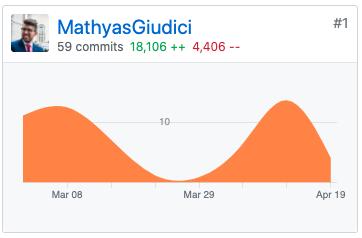
\includegraphics[width=.45\textwidth]{./img/effort/moqa-stat1.png}
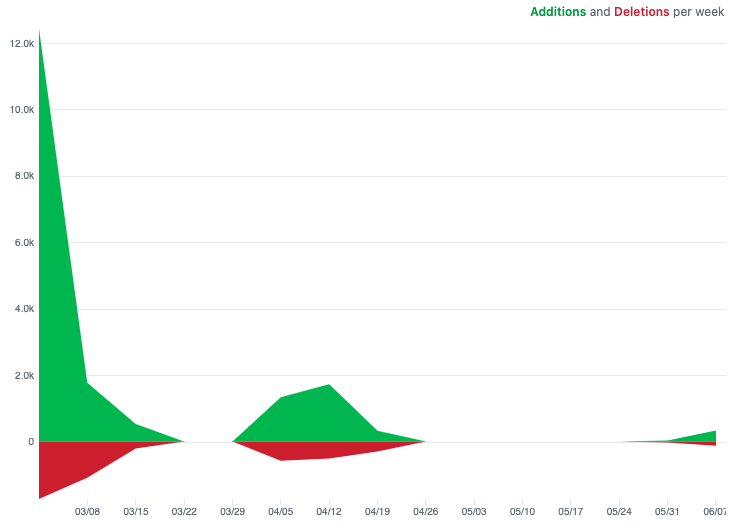
\includegraphics[width=.45\textwidth]{./img/effort/moqa-stat2.png}
\hspace{0.05\linewidth}
\caption{Screenshots from \textit{MOQA} repository on \textit{GitHub}}
\label{img:moqa-stats}
\end{figure}

\begin{figure}[H]
\centering
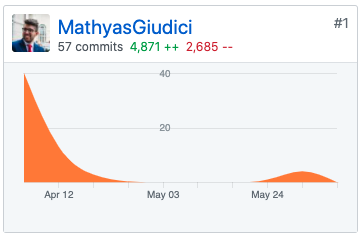
\includegraphics[width=.45\textwidth]{./img/effort/server-stat1.png}
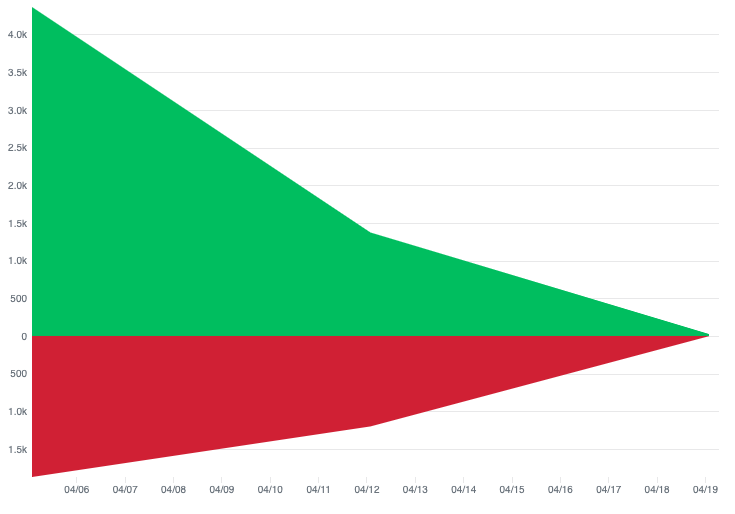
\includegraphics[width=.45\textwidth]{./img/effort/server-stat2.png}
\hspace{0.05\linewidth}
\caption{Screenshots from \textit{Application Server} repository on \textit{GitHub}}
\label{img:moqa-stats}
\end{figure}

\section{Cost Estimation}
In this section is described a cost estimation based on the \textit{COCOMO} method.

The \textit{Constructive Cost Model} (COCOMO) is an algorithmic software cost estimation model developed by Barry W. Boehm.\\
The model uses a basic regression formula with parameters that are derived from historical project data and current project characteristics.\\

COCOMO applies to three classes of software projects:
\begin{itemize}
    \item \textbf{Organic projects} \textit{small} teams with \textit{good} experience working with \textit{less than rigid} requirements;
    \item \textbf{Semi-detached projects} \textit{medium} teams with mixed experience working with a mix of rigid and less than rigid requirements;
    \item \textbf{Embedded projects} projects are developed within a set of \textit{tight} constraints. It is also combination of organic and semi-detached projects.
\end{itemize}

The basic \textit{COCOMO} equations are:
\begin{itemize}
    \item \textbf{Effort Applied}\quad a(KLOC)\textsuperscript{b}
    \item \textbf{Development Time}\quad c(Effort Applied)\textsuperscript{d}
    %\item \textbf{People Required}\quad Effort Applied/Development Time
\end{itemize}

where, \textit{KLOC} is the estimated number of delivered lines (expressed in thousands ) of code for project.\\
\clearpage

The coefficients a, b, c and d are:
\begin{table}[H]
\begin{tabular}{| p{0.5\textwidth} | p{0.1\textwidth} | p{0.1\textwidth} | p{0.1\textwidth} | p{0.1\textwidth} |}
  \hline
  \textbf{Software Project} & \textbf{a} & \textbf{b} & \textbf{c} & \textbf{d}\\ \hline
  Organic       & 2.40 & 1.05 & 2.50 & 0.38 \\ \hline
  Semi-detached & 3.00 & 1.12 & 2.50 & 0.35 \\ \hline
  Embedded      & 3.60 & 1.20 & 2.50 & 0.32 \\ \hline
\end{tabular}
\end{table}

For the project, I decided to select to consider the project as \textit{Semi-detached}.\\
This consideration comes from a consideration about the team (very small I'm alone), the development that is done with \textit{Vue Native} (first time with \textit{Vue Native} but I already know \textit{Vue.js}) and the fact that I never program an \textit{Arduino} board.\\

From the previous section, the reader could see that the KLOC value could be fixed at 15.\\

\[
EFFORT APPLIED = a\left ( KLOC \right ) ^{b} =  3.00 \left ( 6 \right ) ^{1.12} = 22.3
\]

\[
DEVELOPMENT TIME = C\left ( EFFORT APPLIED \right ) ^{d} =  2.50 \left ( 22.3 \right ) ^{0.35} = 7.4
\]

The \textit{COCOMO} method estimates the time of development in more or less 7 months.

